\section{Theorie}
\label{sec:Theorie}

Ziel des Versuchs ist es, das Elastizitätsmodul eines Metalls zu bestimmen und die berechneten Daten mit Literaturwerten abzugleichen.


\subsection{Allgemein}




\subsection{einseitige Einspannung}

\begin{figure}
    \centering
    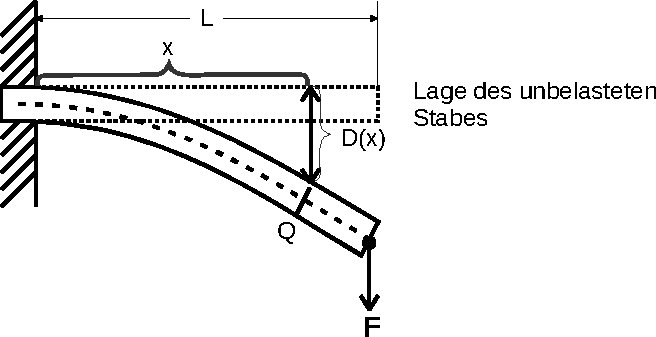
\includegraphics{content/einseitig.pdf}
    \caption{Durchbiegung eines elastischen Stabes bei einseitiger Einspannung \cite[107]{V103}}
    \label{fig:einseits}
  \end{figure}

\subsection{beidseitige Auflage}

\begin{figure}
  \centering
  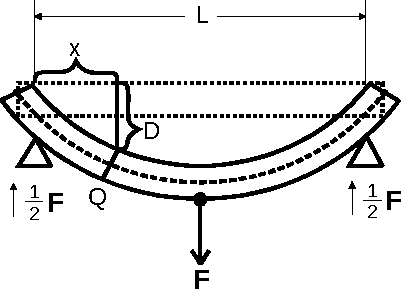
\includegraphics{content/beidseits.pdf}
  \caption{Durchbiegung eines elastischen Stabes bei beidseitiger Auflage\cite[110]{V103}}
  \label{fig:beidseits}
\end{figure}


\cite{sample}
